\section{PHÂN TÍCH CÂU 2}
\addcontentsline{toc}{section}{\numberline {} PHÂN TÍCH CÂU 2}
\setcounter{section}{2}
* \textbf{Truy cập link github để có thể xem code tốt nhất:}  \url{https://github.com/DoTienThanh325/Big_exercise/tree/main/Problem%202}
\subsection{Câu 2 ý 1}
\subsubsection{Ý tưởng làm bài}
Lấy dữ liệu từ bài 1 đưa vào một dataframe lọc ra các cột chỉ số dữ liệu dưới dạng number. Duyệt qua các cột mỗi cột sắp xếp lại theo thứ tự giảm dần của chỉ số lấy ra ba cầu thủ đầu lưu vào file theo yêu cầu đề bài sau đó lại sắp xếp theo thứ tự tăng dần của các chỉ số của cột đó và lấy ba cầu thủ đầu để đưa vào file
\subsubsection{Phân tích code câu 2 ý 1}
    \begin{figure}[H]
        \centering
        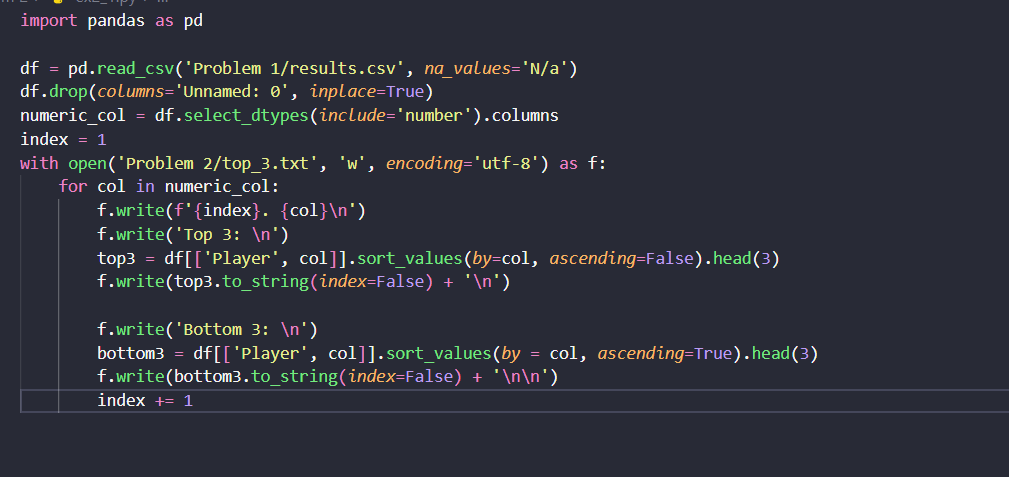
\includegraphics[width=1\linewidth]{img/2_1.png}
    \end{figure}
    - Lấy dữ liệu câu 1 thu được đưa vào dataframe \textbf{df} chuyển tất cả các chuỗi 'N/a' về dạng na bằng câu lệnh: \textbf{df = pd.read\_csv('Problem 1/results.csv', na\_values='N/a')}.\\
    - Loại bỏ cột 'Unnamed: 0' (Là cột index lưu từ câu 1): \textbf{df.drop(columns='Unnamed: 0', inplace=True)}.\\
    - Lấy ra list các cột có dữ liệu dạng số lưu vào \textbf{numeric\_col}: \\ \textbf{numeric\_col = df.select\_dtypes(include='number').columns}
    - Khởi tạo biến index bằng 1 để đánh dấu index các cột chỉ số.\\
    - Mở file để lưu dữ liệu phân tích vào:\\ \textbf{with open('Problem 2/top\_3.txt', 'w', encoding='utf-8') as f:}. \\
    - Dùng vòng \textbf{for} duyệt qua từng cột một, tại mỗi cột:
    \begin{itemize}
        \item Tìm ra ba cầu thủ có chỉ số cao nhất bằng cách sắp xếp dựa vào chỉ số của cột theo chiều giảm dần và đưa vào file:
        \begin{figure}[H]
            \centering
            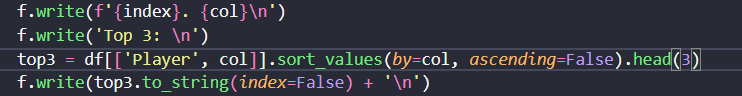
\includegraphics[width=1\linewidth]{img/top3.png}
        \end{figure}
        \item Tìm ra ba cầu thủ có chỉ số thấp nhất bằng cách sắp xếp dựa vào chỉ số của cột theo chiều tăng dần và đưa vào file:
        \begin{figure}[H]
            \centering
            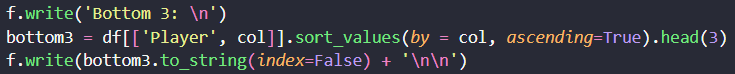
\includegraphics[width=1\linewidth]{img/bottom3.png}
        \end{figure}
    \end{itemize}
    - Sau cột ta lại tăng biến index lên một đơn vị.\\
\subsection{Câu 2 ý 2}
\subsubsection{Ý tưởng làm bài}
Lấy dữ liệu từ bài 1 đưa vào một dataframe lọc ra các cột chỉ số dữ liệu dưới dạng number. Tạo dictionary all\_team để lưu trữ dữ liệu của toàn bộ các đội bóng và có 'Team': 'all' duyệt qua các cột dữ liệu bên trên tính median, mean, std của từng cột và đưa vào dictionary với keys phù hợp sau đó đấy dictionary đó vào một list tổng. Với từng câu lạc bộ ta lấy tất cả cầu thủ thuộc đội bóng đưa vào một dataframe và làm tương tự như toàn giải đấu sau đó cũng đưa vào list tổng. Cuối cùng chuyển list tổng sang dạng dataframe và đấy vào file csv.
\subsubsection{Phân tích code câu 2 ý 2}
    \begin{figure}[H]
        \centering
        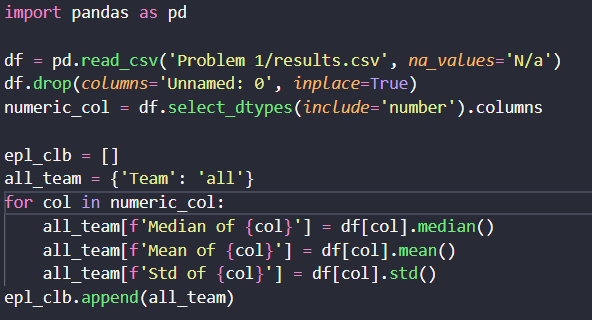
\includegraphics[width=1\linewidth]{img/2_2-1.png}
    \end{figure}
    - Lấy dữ liệu của file csv và chỉnh sửa giống ý 1.\\
    - Khởi tạo một list rỗng: \textbf{epl\_clb = []}
    - Tạo một dictionary có 1 keys là \textbf{Team} và values là \textbf{all}: \textbf{all\_team = \{'Team': 'all'\}}.\\
    - Duyệt qua từng cột của \textbf{numeric\_col}, mỗi cột tạo key và value tương ứng cho dictionary \textbf{all\_team}: \begin{verbatim}
        all_team[f'Median of {col}'] = df[col].median()
        all_team[f'Mean of {col}'] = df[col].mean()
        all_team[f'Std of {col}'] = df[col].std()
    \end{verbatim}
    - Thêm dictionary all\_team vào list epl\_clb: \textbf{epl\_clb.append(all\_team)}
    \begin{figure}[H]
        \centering
        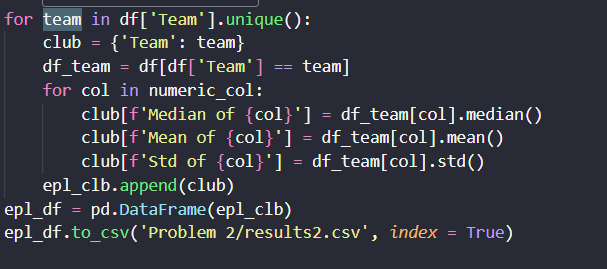
\includegraphics[width=1\linewidth]{img/2_2-2.png}
    \end{figure}
    - \textbf{for team in df['Team'].unique():}: Duyệt qua từng câu lạc bộ một.
    \begin{itemize}
        \item Mỗi câu lạc bộ tạo một dictionary là \textbf{club} với cặp key value đầu là \textbf{'Team': team} và tạo ra một dataframe lưu trữ toàn bộ cầu thủ của câu lạc bộ đó:
        \begin{verbatim}
            club = {'Team': team}
            df_team = df[df['Team'] == team]
        \end{verbatim}
        \item Duyệt qua từng cột và làm tương tự như toàn giải
        \begin{verbatim}
            for col in numeric_col:
                club[f'Median of {col}'] = df_team[col].median()
                club[f'Mean of {col}'] = df_team[col].mean()
                club[f'Std of {col}'] = df_team[col].std()
            epl_clb.append(club)
        \end{verbatim}
    \end{itemize}
    - Cuối cùng đưa list về dạng dataframe và lưu vào file csv:
    \begin{verbatim}
        epl_df = pd.DataFrame(epl_clb)
        epl_df.to_csv('Problem 2/results2.csv', index = True)
    \end{verbatim}

\subsection{Câu 2 ý 3}
\subsubsection{Ý tưởng làm bài}
Lấy những dữ liệu cột dưới dạng số sau đó dùng thư viện matplotlib để vẽ. Dùng subplots để có thể vẽ nhiều biểu đồ cùng một lúc
\subsubsection{Phân tích code câu 2 ý 3}
    \begin{figure}[H]
        \centering
        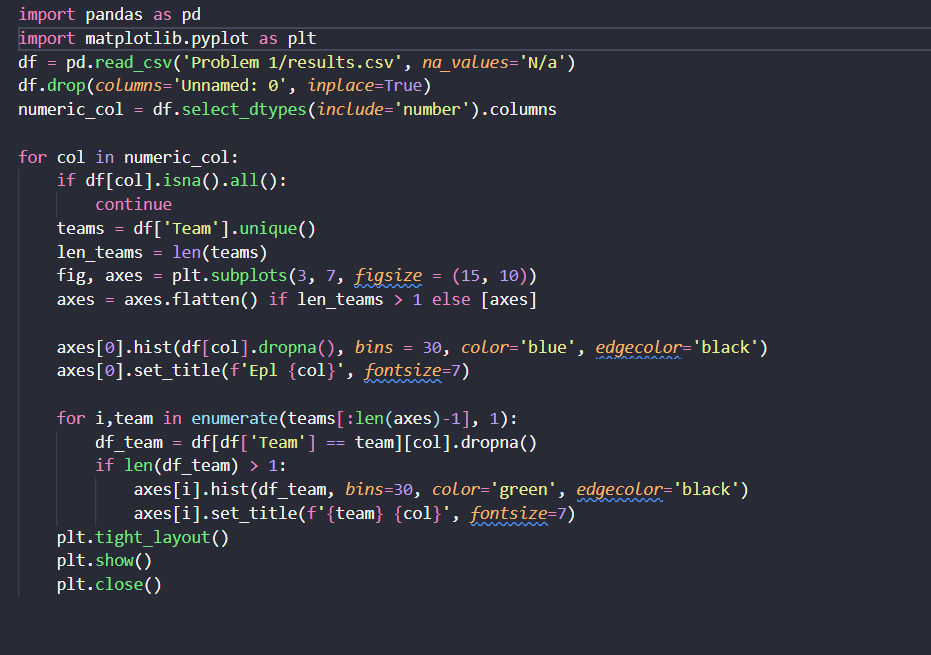
\includegraphics[width=1\linewidth]{img/2_3.png}
    \end{figure}
    - Đọc và xử lý dữ liệu như hai ý trên của câu 2.\\
    - Duyệt qua các cột:
    \begin{itemize}
        \item Nếu cột toàn \textbf{na} ta sẽ chuyển sang cột khác:
        \begin{verbatim}
        for col in numeric_col:
            if df[col].isna().all(): continue
        \end{verbatim}
        \item \textbf{teams = df['Team'].unique()}: Lấy danh sách các đội bóng không trùng trong cột 'Team'.
        \item \textbf{fig, axes = plt.subplots(3, 7, figsize=(15, 10))}: Tạo ra một figure với 3 hàng, 7 cột ô (tức là 21 ô) để vẽ các biểu đồ nhỏ (subplots).
        \item \textbf{axes = axes.flatten() if len\_teams > 1 else [axes]}: Vì axes ban đầu là một mảng 2D (3x7), nên bẻ phẳng thành 1D list cho dễ lặp. Còn nếu chỉ có 1 team thì axes không phải mảng, nên cho vào list để tránh lỗi.
        \item \textbf{axes[0].hist(df[col].dropna(), bins = 30, color='blue', edgecolor='black')}: Vẽ biểu đồ tần suất của cả giải trên subplot đầu tiên \textbf{axes[0]}. \textbf{dropna()} để loại bỏ giá trị NaN (trống) trước khi vẽ. \textbf{bins=30}: chia thành 30 cột nhỏ.  \textbf{color='blue'}: màu bên trong cột.  \textbf{edgecolor='black'}: viền cột màu đen.
        \item \textbf{axes[0].set\_title(f'Epl {col}', fontsize=7)}: Gắn tựa đề cho subplot. . \textbf{fontsize=7}: cỡ chữ cho tiêu đề.
        \item \textbf{enumerate(teams[:len(axes)-1], 1)}: Bắt đầu từ i = 1 (vì axes[0] đã dùng để vẽ EPL tổng). teams[:len(axes)-1]: tránh bị lỗi nếu số đội > số subplot.
        \item \textbf{df\_team = df[df['Team'] == team][col].dropna()}: Lọc ra dữ liệu cột col của từng đội. \textbf{dropna()} để không vẽ các giá trị thiếu.
        \item Đoạn code:
    \begin{verbatim}
    if len(df_team) > 1:
        axes[i].hist(df_team, bins=30, color='green', edgecolor='black')
        axes[i].set_title(f'{team} {col}', fontsize=7)
    \end{verbatim}
        kiểm tra \textbf{len(df\_team)} > 1 không để đảm bảo không lỗi. Hai câu sau giống như cách vễ biểu đồ tổng khác ở màu của cột là màu xanh lá cây.
        \item \textbf{plt.tight\_layout()}: Loại bỏ các biểu đồ rỗng.
        \item \textbf{plt.show()}: Hiển thị các biểu đồ khi run code.
        \item \textbf{plt.close()}: Xóa figure đã vẽ xong ra khỏi bộ nhớ.
    \end{itemize}
\subsection{Câu 2 ý 4} 
\subsubsection{Ý tưởng làm bài}
Tính trung bình cộng tất cả các chỉ số dưới dạng số liệu chọn ra đội đứng đầu ở nhiều nhất các chỉ số là đội có màn trình diễn tốt nhất.
\subsubsection{Phân tích code câu 2 ý 4}
\begin{figure}[H]
    \centering
    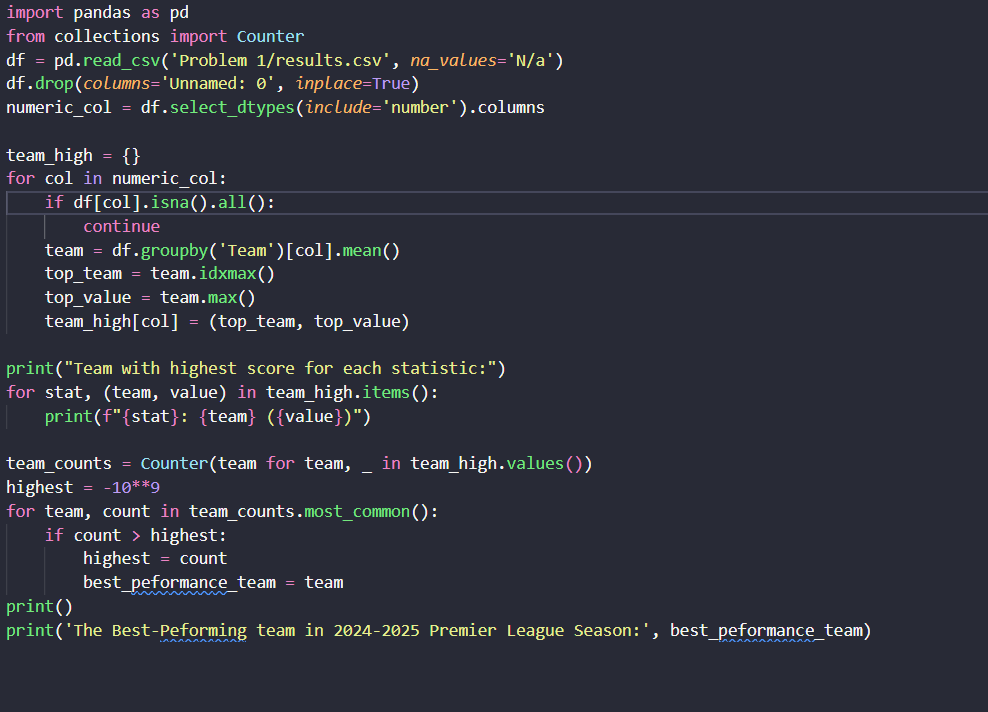
\includegraphics[width=1\linewidth]{img/2-4.png}
\end{figure}
- Xử lý dữ liệu như các ý trên của câu 2.\\
- \textbf{for col in numeric\_col:}: Duyệt qua các cột giá trị.\\
- \textbf{if df[col].isna().all(): continue}: Cột nào toàn giá trị NaN thì chuyển qua cột khác.\\
- \textbf{team = df.groupby('Team')[col].mean()}: Sử dụng hàm \textbf{groupby()} và hàm \textbf{mean()} để tính trung bình cộng các chỉ số của từng đội.\\
- \textbf{top\_team = team.idxmax()}: Dùng hàm \textbf{idxmax()} tìm ra đội có chỉ số trung bình cộng cao nhất.\\
- \textbf{top\_value = team.max()}: Dùng hàm \textbf{max()} tìm ra chỉ số cao nhất.\\
- \textbf{team\_high[col] = (top\_team, top\_value)}: Dùng dictionary để lưu trữ với key là tên cột và value là một tuple gồm hai giá trị \textbf{top\_team} và \textbf{top\_value}.\\
- Đoạn code:
    \begin{verbatim}
    print("Team with highest score for each statistic:")
    for stat, (team, value) in team_high.items():
        print(f"{stat}: {team} ({value})")
    \end{verbatim}
    \begin{itemize}
        \item Dùng để in các đội đứng đầu tại chỉ số và chỉ số đó
    \end{itemize}
- \textbf{team\_counts = Counter(team for team, \_ in team\_high.values())}: Tạo mảng đếm để đếm xem mỗi đội đứng đầu mỗi chỉ số bao lần, đội đứng đầu nhiều nhất là đội có best-peforming.\\
- Đoạn code:
    \begin{verbatim}
    highest = -10**9
    for team, count in team_counts.most_common():
        if count > highest:
            highest = count
            best_peformance_team = team 
    \end{verbatim}
    \begin{itemize}
        \item Đoạn code này dùng để tìm đội có số lần đứng đầu và gán cho biến \textbf{best\_peformance\_team} là đội bóng có số lần đứng đầu nhiều nhất.
    \end{itemize}